\documentclass[main.tex]{subfiles}

\begin{document}
\sloppy


\vspace{1.0cm}

\section{Implementazione di nuove funzionalità alle fixtures}\label{sec:NewFeatures}
Una volta creata una pipeline di rendering, sistemata la gerarchia dei componenti e fatta funzionare l'interpolazione è possibile finalmente aggiungere nuove features alle fixture virtuali. Come visto nel capitolo \ref{sec:RenderingPipeline}, per aggiungere una nuova feature bisogna:
\begin{itemize}
	\item Implementarla come codice HLSL.
	\item Implementarla come MaterialFunction.
	\item Aggiungerla al generatore di codice HLSL.
	\item Aggiungerla al generatore della pipeline per il rendering del materiale Light e Lens.
    \item Creare il FixtureComponent che la gestisce.
\end{itemize}
In questo capitolo non tratteremo mai il secondo punto poiché consiste nella rimplementazione come MaterialExpression del codice già visto in HLSL.

\subsection{Sagomatori}\label{subsec:5_shaper}
\begin{figure}[H]
    \centering
    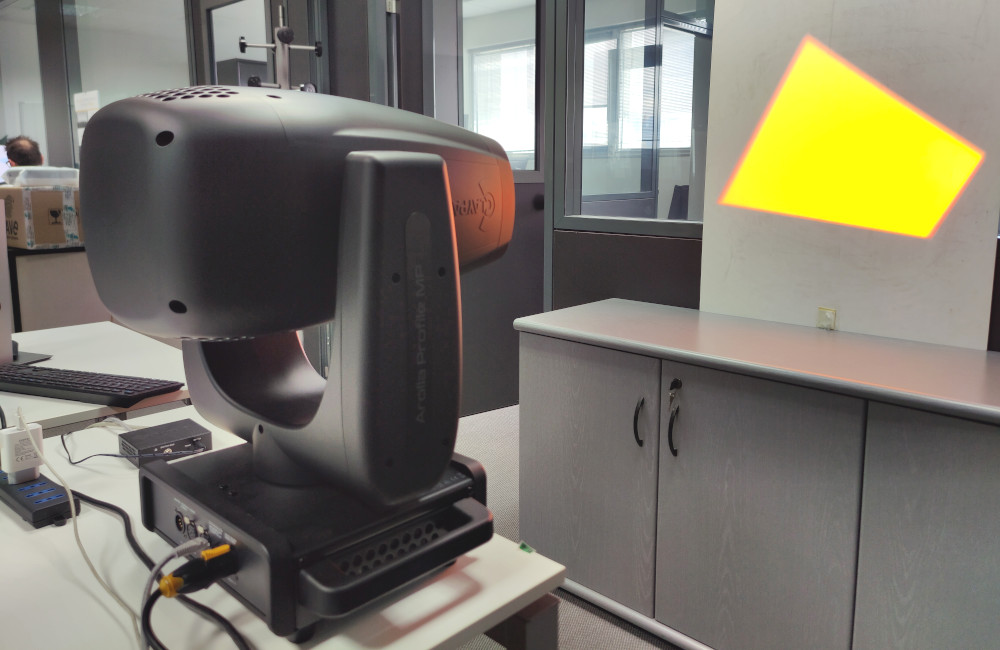
\includegraphics[width=.8\linewidth]{img/newFeatures/shaper.jpg}
    \caption{Sagomatore in azione.}
    \label{fig:5_shaper}
\end{figure}
Il sistema dei sagomatori (detto anche \say{framing system} oppure \say{shaper}) consiste in un modulo composto da 4 lame (dette anche \say{bandiere}) che possono immettersi ed inclinasi singolarmente all'interno del fascio di luce. Inoltre, l'intero modulo può roteare, muovendo contemporaneamente la direzione in cui si immettono tutte le lame si immettono.
%TODO Esempi con foto
Il controllo della lama può avvenie in due modi:
\begin{itemize}
	\item \textbf{A+B}: Controlliamo singolarmente l'immissione dei due punti estremi della lama ($A$ e $B$). Per avere la lama \say{dritta} Dovremmo avere $A = B$, per inclinarla da un lato basta avere uno dei due valori maggiori dell'altro.
	\item \textbf{A+Rot}: Controlliamo l'immissione della lama ($A$) e separatamente la sua inclinazione ($R$).
\end{itemize}
\begin{figure}[H]
    \centering
    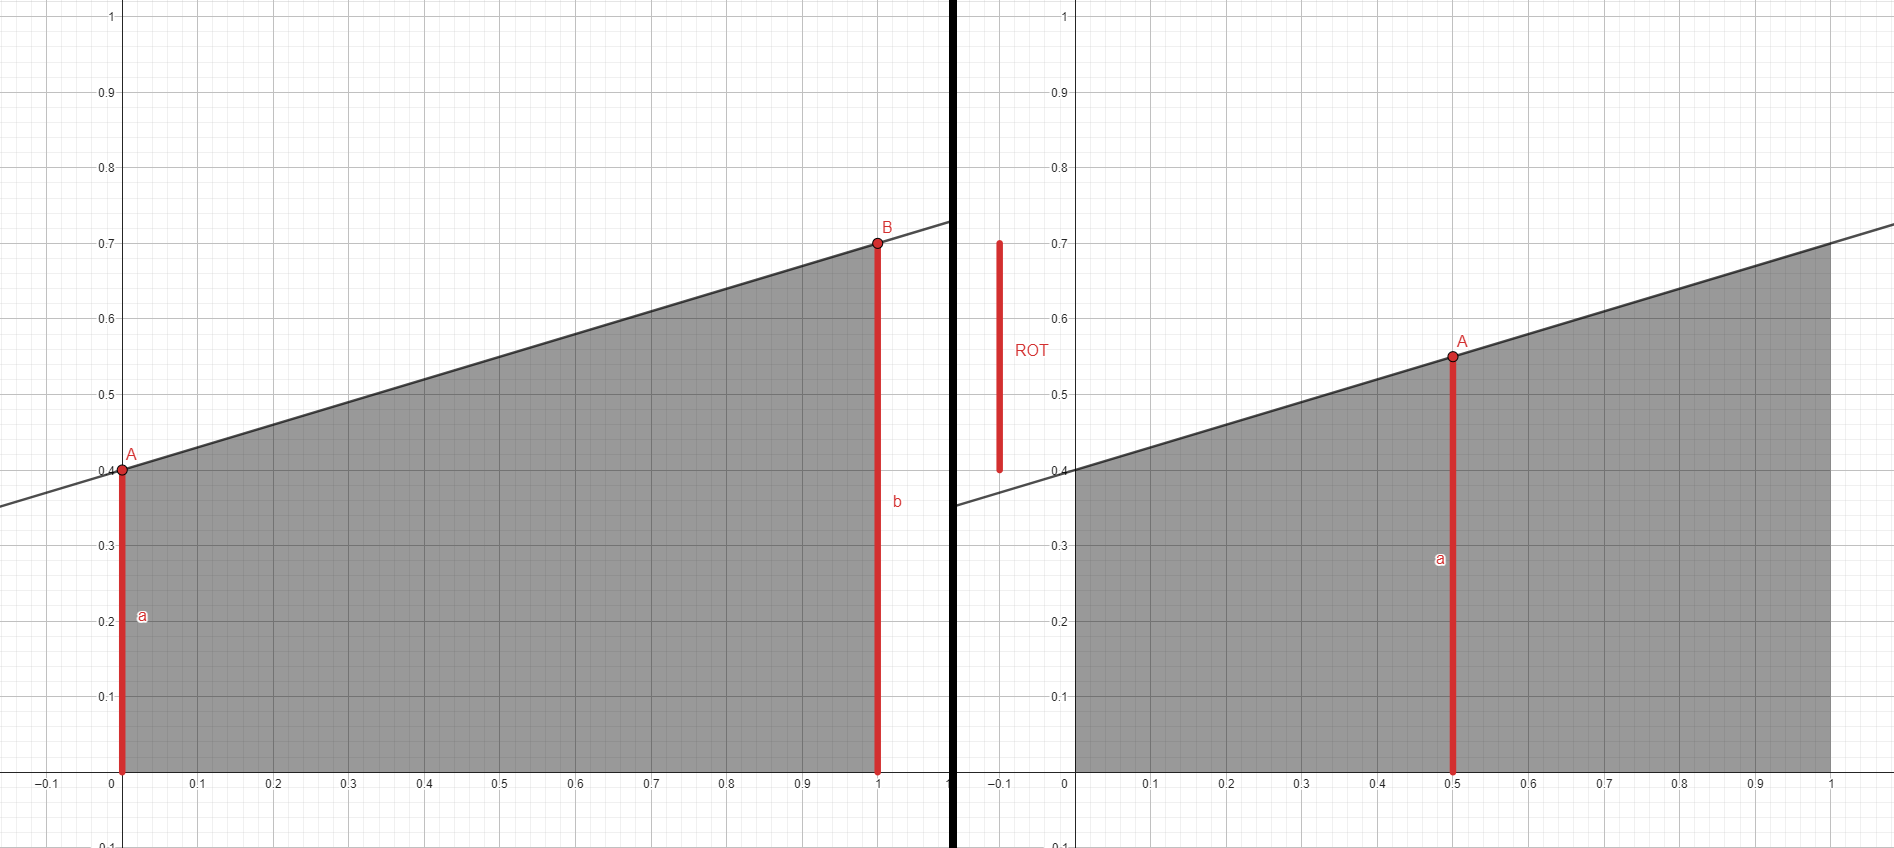
\includegraphics[width=1\linewidth]{img/newFeatures/abVSarot.png}
    \caption{A sinistra, la modalità di controllo \textit{A+B}. A destra, \textit{A+Rot}}
    \label{fig:5_shaperDifferentModes}
\end{figure}

Effettuare il rendering di una funzionalità come lo shaper attraverso texture che vengono roteate e spostate è davvero oneroso in termini computazionali. La scelta migliore è fare il rendering immaginandoci il framing system come delle equazioni matematiche. In generale, il rendering di un materiale avviene effettuando lo stesso calcolo con, in input, differenti coordinate UV, ovvero coordinate bidimensionali normalizzate tra [0, 1] che rappresentano un punto all'interno di una texture. Possiamo immaginare il nostro codice come se fosse inserito in un ciclo for che si scorre \say{tutte} le x e le y comprese tra 0 ed 1, codice che però si occupa di renderizzare una sola UV alla volta. 

\clearpage %TODO CHECK IF IT'S STILL NEEDED
\subsubsection{Idea come formula matematica}\label{subsec:5_1_ShaperMath}
\begin{wrapfigure}{r}{0.45\textwidth}
    \centering
    \captionsetup{justification=centering}
    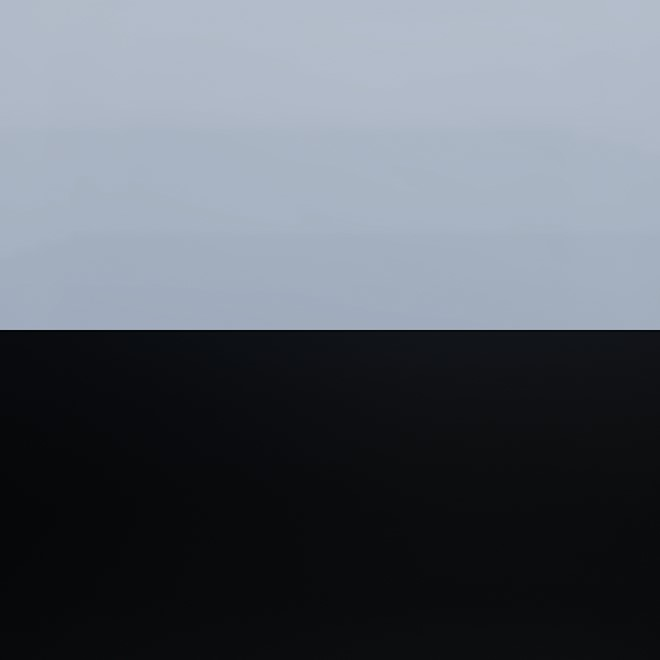
\includegraphics[scale=0.35]{img/newFeatures/eqExample.jpg}
    \caption{Esempio di rendering con il codice \lstinline{return y > 0.5;}}
    \label{fig:5_eqExample}
\end{wrapfigure}
Se immaginiamo quindi una singola lama come una equazione matematica, possiamo renderizzarla controllando semplicemente se la Y della coordinata UV che stiamo renderizzando in quel momento si trova sopra o sotto l'equazione. Il nostro lavoro diventa quindi generare la corretta equazione matematica in base agli input $A$ e $B$ o $R$.

Per trovare l'equazione della retta quando facciamo il sample A+B, possiamo ricorrere alla formula per ottenere l'equazione di una retta passante per due punti:
\[m = \frac{y_2 - y_1}{x_2 - x_1}\]
Immaginiamo che i valori di $A$ e $B$ corrispondano alle loro y, che $A$ si trovi a coordinate $x = 0$ (completamente a sinistra della texture) e che $B$ si trovi a $x = 1$ (completamente a destra della texture). La formula sarà uguale a:
\[m = \frac{y_B - y_A}{x_B - x_A} = \frac{B - A}{1 - 0} = B - A\]
In questo modo generiamo il coefficiente di una retta che però ha sempre origine in $(0, 0)$. Nella realtà, ciò che abbiamo appena creato è un sagomatore in cui solamente il valore B \say{funziona}. Per far \say{funzionare} anche il valore $A$, basta aggiungerlo come termine noto del'equazione.

Come scritto sopra, per generare una flag bisogna controllare quando stiamo \say{sopra} questa equazione, rendendola quindi uguale a:
\[y > x(B - A) + A\]
\newline

Per effettuare, invece, il sampling di una flag A+Rot, possiamo utilizzare $A$ come termine noto, e convertire $R$ da gradi alla relativa tangente trigonometrica in modo da avere direttamente il coefficiente della retta. Poiché vogliamo però inclinare questa retta usando come punto di rotazione il suo centro ($x = 0.5$) e non la sua origine ($x = 0$), dobbiamo modificare il termine noto in base al coefficiente: più il coefficiente è elevato (e più la retta sarà quindi inclinata crescendo da sinistra verso destra) e più il termine noto dovrà calare. Considerando la sezione della retta compresa tra $x = [0, 1]$, la tangente di $R$, essendo direttamente uguale al coefficiente della retta, è anche uguale alla differenza tra il valore della $y$ quando la retta avrà $x = 0$ e quando avrà $x = 1$ (Visibile nella seconda immagine della figura \ref{fig:5_shaperDifferentModes}). Al centro di questa sezione (quando $x = 0.5$) la differenza con i due estremi sarà quindi uguale a $\frac{tan(R)}{2}$, ovvero esattamente il valore da sottrarre al termine noto per mantenere centrale il punto di rotazione della retta. La formula finale dell'equazione sarà quindi:
\[y > \tan(R)x + (a - \frac{\tan(R)}{2})\]

Come le ruote, anche il framing system deve implementare il frost. Piuttosto di applicare un filtro di blur al framing system già renderizzato, è preferibile in termini di peso computazionale implementare una sfocatura come formula matematica direttamente nel precedente rendering. L'idea è quella di utilizzare il valore del frost per definire la dimensione di una zona di sfumatura intorno alla retta. La prima operazione che viene effettuata è trovare la distanza della coordinata UV che stiamo renderizzando dalla retta. Questa operazione viene approssimata come la distanza assoluta ($d$) tra la $y$ della coordinata UV e la $y$ della retta per ogni $x$.
\[d = \abs{y - g(x)}\]
Dove $g(x)$ è la funzione matematica scelta per effettuare il sample della flag.

Lo step suguente è trasformare il valore di frost ($f$) dentro una semplice funzione di remapping:
\[remapFrost(f) \coloneqq f * 0.05 + 0.002\]
Dove $0.05$ e $0.002$ sono valori magici trovati dopo discreti tentativi di try and error.

Successivamente viene applicata un'altra funzione di remapping sulla distanza, in modo che sia scalata all'interno del valore frost:
\[remapDist(d, f) \coloneqq 
	\begin{dcases}
		\hfil 1 & \text{se } d > remapFrost(f)\\
		\frac{d}{remapFrost(f)} & \text{altrimenti}
	\end{dcases}
\]

Poiché $d$ all'inizio viene calcolata come distanza assoluta dalla retta, con quanto definito fin'ora avremo una figura nera che si dissolve andando verso il bianco quando siamo abbastanza vicini alla retta stessa. Dobbiamo invece fare in modo che la dissolvenza parta da bianco, diventi grigia in corrispondenza della retta, e nera dopo la stessa:
\[fade(d, f) \coloneqq 
	\begin{dcases}
		\hfil	 \frac{remapDist(d, f)}{2} & \text{se } y > g(x)\\
				-\frac{remapDist(d, f)}{2} & \text{altrimenti}
	\end{dcases}
\]
\newline

\begin{wrapfigure}{r}{0.45\textwidth}
    \centering
    \captionsetup{justification=centering}
    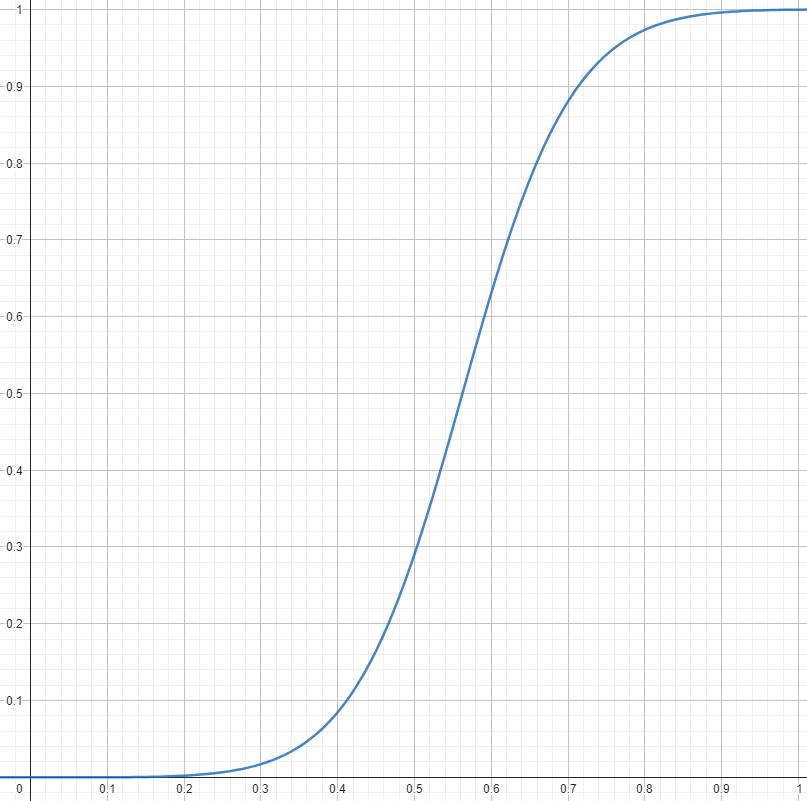
\includegraphics[scale=0.35]{img/newFeatures/sCurve.png}
    \caption{Funzione $sCurve(v)$}
    \label{fig:5_sCurve}
\end{wrapfigure}
Per un effetto ottico in cui è molto più semplice distinguere gradazioni differenti di colori scuri rispetto a gradazioni differenti di colori chiari, applicando il frost sembrerà che il valore del sagomatore si sposti verso il basso, come in figura \ref{fig:5_shaperFixes}. Per compensare ciò, il risultato finale calcolato in precedenza, viene passato all'interno di un'ultima funzione di remapping: quello che vogliamo è creare una curva ad S (figura \ref{fig:5_sCurve}), in modo che la dissolvenza avvenga repentinamente al centro dei nostri valori piuttosto che linearmente da 0 ad 1.
\[sCurve(v) \coloneqq \frac{1}{1 + (\frac{v}{1.125 - v})^{-4}}\]
Dove i valori all'interno della frazione e l'esponenziale sono ottenuti via try ed error. Il valore $1.125$ serve per sbilanciare verso destra la curva, l'esponenziale per regolarne l'ampiezza.
\begin{figure}[H]
    \centering
    
\includegraphics[width=1\linewidth]{img/newFeatures/shaperFixes.jpg}
    \caption{Da destra verso sinistra: flag senza frost; flag con frost e passaggio dei valori lineare tra 0 ed 1; flag con frost e con la funzione $sCurve(v)$ applicata.}
    \label{fig:5_shaperFixes}
\end{figure}


Con il frost abilitato si verifica anche un altro problema: Quando una flag è completamente aperta oppure è completamente chiusa, vedremo comunque renderizzata la sfumatura del frost, piuttosto che avere una figura completamente bianca o nera. Le fixture reali risolvono questo problema facendo muovere le bandiere oltre i limiti di apertura e chiusura. Creiamo quindi due funzioni da anteporre a tutti i calcoli per questa feature, che modifichino il valore di $A$ e di $B$. 
\[frostLimit(f) \coloneqq 
	\begin{dcases}
		\hfil f & \text{se } f < 0.2\\
		0.2 & \text{altrimenti}
	\end{dcases}
\]
\[remapABposition(x, f) \coloneqq x(2 * frostLimit(f) + 1) - frostLimit(f)\]
% x = max(frost, 0.2)
% res = (inp * (x * 2 + 1)) - x
Questa funzione si occupa di rimappare il valore di $A$ o di $B$ all'interno di un range via via più piccolo man mano che cresce il valore di frost. Viene anche imposto un valore minimo di frost, in modo da emulare l'effetto della lama che supera i limiti di apertura e chiusura anche quando è disattivato.
\newline

La direzione di ogni singola bandiera, così come la rotazione dell'intero framing system viene implementata come un'unica funzione \cite{UVrotation} che prende in input la somma dei due valori:
\[finalAngle = direction + framingSystemAngle\]
Dove $direction$ può essere uguale a 0, 90, 180 o 270 gradi. La rotazione viene effettuata trasformando i valori UV prima di qualsiasi altro calcolo effettuato per il sample di ogni singola blade.
\[rotateUV(a) \coloneqq 
	\begin{bmatrix}
		\cos(a)(x - \frac{1}{2}) + \sin(a)(y - \frac{1}{2}) + x \\
		\cos(a)(y - \frac{1}{2}) + \sin(a)(x - \frac{1}{2}) + y
	\end{bmatrix}
\]
Dove $a$ corrisponde ai gradi di rotazione in input.

\subsubsection{Generazione codice HLSL ed inserimento nel materiale Beam}\label{subsec:5_1_ShaperHlsl}
\lstset{language=glsl}
Le funzioni $fade$, $sCurve$ e $rotateUV$ sono state scritte in maniera generica poiché sono utili anche nel sample di altre features (Ad esempio, l'iris \ref{subsec:5_Iris}). Le funzioni di remapping sono state, invece, accorpate tra di loro. Le condizioni sono implementate con la formula \lstinline{float b = /*boolean expression*/; float f = b * x + (1 - b) * y;} per ridurre la branch divergence nell'esecuzione del codice hlsl.
\begin{lstlisting}
float sCurve(float f){
	const float exp = -4;
	f = saturate(f);
	return 1 / (1 + pow((f / (1.125 - f)), exp));
}

void rotateUV(float2 texCoor, float rads, out float x, out float y) {
	float c = cos(rads);
	float s = sin(rads);
	x = c * (texCoor.x - 0.5) + s * (texCoor.y - 0.5) + 0.5;
	y = s * (texCoor.x - 0.5) - c * (texCoor.y - 0.5) + 0.5;
}

float fade(float passed, float d, float frost){
	float max = 0.05 * frost + 0.002;
	float clamp = d > max;
	d = clamp + (1 - clamp) * (d / max);

	return sCurve((passed * 2 - 1) * (d / 2) + 0.5);
}
\end{lstlisting}

Il codice per fare il sample delle due differenti modalità è implementato come due funzioni separate, seppur molto simili:
\begin{lstlisting}
float sampleBladeAB(float2 texCoor, float a, float b,
		float orientationRads, float frost){
	float x, y;
	rotateUV(texCoor, orientationRads, x, y);
	float m = b - a;
	float eq = (x * m) + a;
	float d = abs(y - eq);
	float passed = y > eq;
	return fade(passed, d, frost);
}
float sampleBladeARot(float2 texCoor, float a, float rotRads,
		float orientationRads, float frost){
	float x, y;
	rotateUV(texCoor, orientationRads, x, y);
	float m = rotRads * x;
	float eq = m - (rotRads * 0.5) + a;
	float d = abs(y - eq);
	float passed = y > eq;
	return fade(passed, d, frost);
}
\end{lstlisting}


Nel costruttore della \lstinline{CPGDTFRenderPipelineBuilder}, all'interno del for finale, è stato aggiunto del codice che ricerca i componenti di tipo ShaperFixtureComponent e li aggiunge ad un array di bandiere.
\lstset{language=UEcpp}
\begin{lstlisting}
auto shaper = Cast<UCPGDTFShaperFixtureComponent>(components[i]);
if (shaper != nullptr) {
    shapers.Add(shaper);
    continue;
}
\end{lstlisting}

Il codice per la generazione del codice HLSL in se è molto semplice. Si prende in input un array di ShaperFixtureComponent già instanziati e per ciascuno controlla se sono in modalità A+B oppure A+Rot, e seleziona la relativa chiamata a funzione corretta.
\begin{lstlisting}
for (int i = 0; i < mShapers.Num(); i++) {
    FString orientationVarName =
        CPGDTFRenderPipelineBuilder::getInputBladeOrientationName(
            mShapers[i]->getOrientation()
        );
    FString bRotVarName =
        CPGDTFRenderPipelineBuilder::getInputBladeABRotName(
            false, mShapers[i]->getOrientation()
        );
    FString aVarName =
        CPGDTFRenderPipelineBuilder::getInputBladeABRotName(
            true, mShapers[i]->getOrientation()
        );

    if (mShapers[i]->isInAbMode()) { //a+b mode
        placeholderCode = placeholderCode + FString::Format(*textAdd, {
            FString::Printf(
                TEXT("sampleBladeAB(pos.xy, %s, %s, %s, %s)"),
            *aVarName, *bRotVarName, *orientationVarName, *frostVarName)
        });
    } else { //a + rot mode
        placeholderCode = placeholderCode + FString::Format(*textAdd, {
            FString::Printf(
                TEXT("sampleBladeARot(pos.xy, %s, %s, %s, %s)"),
            *aVarName, *bRotVarName, *orientationVarName, *frostVarName)
        });
    }
}
\end{lstlisting}

La funzione $remapABposition$ è stata implementata come MaterialFunction invece che come codice hlsl, in modo che possa venire ottimizzata automaticamente da UnrealEngine \cite{hlslNoOptimize}. Inoltre è stata creata un'altra MaterialFunction (ConvertRot) che si occupa di convertire i gradi in radianti e di ottenerne il valore della tangente. L'inserimento degli input e dei parametri nel materiale Beam inizia caricandosi queste due MaterialFunction.
\begin{lstlisting}
UMaterialFunctionInterface* mfShaperConvertBladePosition =
    Cast<UMaterialFunctionInterface>(
        FCPGDTFImporterUtils::LoadObjectByPath(
            mfShaperConvertBladePositionPath
        )
    );
UMaterialFunctionInterface* mfShaperConvertRot =
    Cast<UMaterialFunctionInterface>(
        FCPGDTFImporterUtils::LoadObjectByPath(
            mfShaperConvertRotPath
        )
    );
\end{lstlisting}
Successivamente viene creata una lambda che si occuperà di aggiungere effettivamente un parametro al materiale.
\begin{lstlisting}
const std::function<void(FString, FString, bool)>
    addABRotParameterToBeamPipeline = [&](
        FString paramName, //Nome del parametro del materiale
        FString variableName, //Nome della variabile della CE
        bool isRot //Se true, il parametro corrisponde al valore "rot"
    ) {
    //...
}
\end{lstlisting}
Infine si scorre la lista degli shaper e per ciascuno aggiunge tre parametri, A, B/Rot e rotazione. Quando viene generato il parametro B/Rot si controlla la modalità dello shaper attraverso la funzione \lstinline{isInAbMode()}.
\begin{lstlisting}
for (UCPGDTFShaperFixtureComponent *shaper : shapers) {
    int orientation = shaper->getOrientation(); //ID della flag

    addABRotParameterToBeamPipeline( //Generazione parametro A
        getBladeABRotParamName(true, orientation),
        getInputBladeABRotName(true, orientation),
        false
    );
    addABRotParameterToBeamPipeline( //Generazione parametro B/Rot
        getBladeABRotParamName(false, orientation),
        getInputBladeABRotName(false, orientation),
        !shaper->isInAbMode()
    );
    addScalarInputToBeamPipeline( //Parametro per la rotazione
        dstMaterial,
        getBladeOrientationParamName(orientation),
        getInputBladeOrientationName(orientation),
        meCustom, meBlocksMover
    );
}
\end{lstlisting}
Dove \lstinline{getBladeABRotParamName()} e \lstinline{getInputBladeABRotName()} prendono \lstinline{true} se stiamo generando il parametro A o \lstinline{false} se stiamo generando il parametro B o Rot (I due valori condividono lo stesso parametro). \newline

La lambda citata sopra si occupa come prima cosa di generare il parametro effettivo.
\begin{lstlisting}
    UMaterialExpressionScalarParameter* param =
        generateMaterialExpression<UMaterialExpressionScalarParameter>(
            dstMaterial
        );
    param->ParameterName = FName(*paramName);
    param->Group = FName(TEXT("Runtime Parameters"));
    param->SortPriority = 5;
    param->DefaultValue = 0;
    dstMaterial->GetEditorOnlyData()->ExpressionCollection.
        AddExpression(param);
\end{lstlisting}
Successivamente crea, imposta, collega e sposta la MaterialFunctionCall in base alla modalità selezionata.
\begin{lstlisting}
UMaterialExpressionMaterialFunctionCall* mfCall = 
    generateMaterialExpression<UMaterialExpressionMaterialFunctionCall>(
        dstMaterial
    );
dstMaterial->GetEditorOnlyData()->ExpressionCollection.
    AddExpression(mfCall);
if (isRot) {
    mfCall->SetMaterialFunction(mfShaperConvertRot);
} else {
    mfCall->SetMaterialFunction(mfShaperConvertBladePosition);
    mfCall->FunctionInputs[1].Input.Connect(0, scalarFrost); //Frost
}
mfCall->FunctionInputs[0].Input.Connect(0, param); //Value

mfCall->MaterialExpressionEditorX =
    meBlocksMover->getCurrentX()+ BEAM_EDITOR_BLOCK_DISTANCE_X;
mfCall->MaterialExpressionEditorY =
    meBlocksMover->getCurrentY() + EDITOR_MINI_BLOCK_SIZE;
meBlocksMover->moveMaterialExpression(param, EDITOR_SCALAR_PARAM_SIZE);
\end{lstlisting}
Infine, genera un input sulla CustomExpression e lo collega alla precedente MaterialFunctionCall.
\begin{lstlisting}
FCustomInput input;
input.InputName = FName(*variableName);
input.Input.Connect(0, mfCall);
meCustom->Inputs.Add(input);
\end{lstlisting}

\subsubsection{Generazione nella RenderingPipeline per Light e Lens}\label{subsec:5_1_ShaperRenderingPipeline}
Come per la generazione del materiale Beam anche qui le varie funzioni descritte nel capitolo \ref{subsec:5_1_ShaperMath} sono state trasformate in MaterialFunctions. Come spiegato nella sezione \ref{sec:RenderingPipeline} tali MaterialFunctions prenderanno in input l'output della precedente, per formare la pipeline di rendering. L'implementazione in se delle MaterialFunctions non viene vista poiché è identica al codice HLSL spiegato nel capitolo precedente, bensì vedremo comunque la parte di generazione della pipeline. \newline

Si effettua un ciclo su tutti gli ShaperFixtureComponent che dobbiamo aggiungere alla pipeline. Per ciascuno, iniziamo con lo generare una MaterialFunctionCall ed impostarne la MaterialFunction in base alla modalità della flag.
\begin{lstlisting}
int orientation = shaper->getOrientation();
UMaterialExpressionMaterialFunctionCall* currentNode =
    generateMaterialExpression<UMaterialExpressionMaterialFunctionCall>(
        dstMaterial
    );
dstMaterialData->ExpressionCollection.AddExpression(currentNode);

if (shaper->isInAbMode()) currentNode->SetMaterialFunction(mfShaperAB);
    else currentNode->SetMaterialFunction(mfShaperARot);
\end{lstlisting}
Successivamente vengono generati e connessi i vari parametri della precedente MaterialFunctionCall.
\begin{lstlisting}
auto aParam = addScalarParameterToMiPipeline(
    dstMaterial,
    getBladeABRotParamName(true, orientation),
    meParamsMover
);
auto bRotParam = addScalarParameterToMiPipeline(
    dstMaterial,
    getBladeABRotParamName(false, orientation),
    meParamsMover
);
auto orientationParam = addScalarParameterToMiPipeline
    dstMaterial,
    getBladeOrientationParamName(orientation),
    meParamsMover
);

currentNode->FunctionInputs[1].Input.Connect(0, previousParameter);
currentNode->FunctionInputs[2].Input.Connect(0, frostParam);
currentNode->FunctionInputs[3].Input.Connect(0, aParam);
currentNode->FunctionInputs[4].Input.Connect(0, bRotParam);
currentNode->FunctionInputs[5].Input.Connect(0, orientationParam);
\end{lstlisting}
Ed infine viene spostata ed impostata come ultimo nodo generato.
\begin{lstlisting}
meModulesMover->moveMaterialExpression(currentNode);
previousParameter = currentNode;
delete meParamsMover;
\end{lstlisting}

\subsubsection{ShaperFixtureComponent}\label{subsec:5_1_ShaperFixtureComponent}
L'implementazione del componente è molto semplice, vista la gerarchia dei componenti che abbiamo creato in precedenza. L'unico codice elaborato presente nel componente si trova nella funzione \lstinline{Setup()}, e si occupa solamente di capire in che modalità il componente viene usato. 

Questa operazione viene effettuata scorrendo tutta la lista di ChannelFunction assegnate al componente, e viene impostata la modalità \say{A+B} ogni qualvolta si incontra un componente B, oppure la modalità \say{A+Rot} ogni qualvolta si incontra un componente Rot.
\begin{lstlisting}
for (Per ogni ChannelFunction cf) {
    auto attrType =
        CPGDTFDescription::GetGDTFAttributeTypeValueFromString(
            cf.Attribute.Name.ToString()
        );

    if (attrType == ECPGDTFAttributeType::Blade_n_Rot) {
        abMode = false;
    } else if (
               attrType == ECPGDTFAttributeType::Blade_n_B
            || attrType == ECPGDTFAttributeType::BladeSoft_n_B
            ) {
        abMode = true;
    }
}
\end{lstlisting}

Di seguito, degli screenshot della classe per mostrare quanto sia semplice implementare nuovi componenti ora che la gerarchia di FixtureComponent è stata rivoluzionata.
\begin{figure}[H]
    \centering
    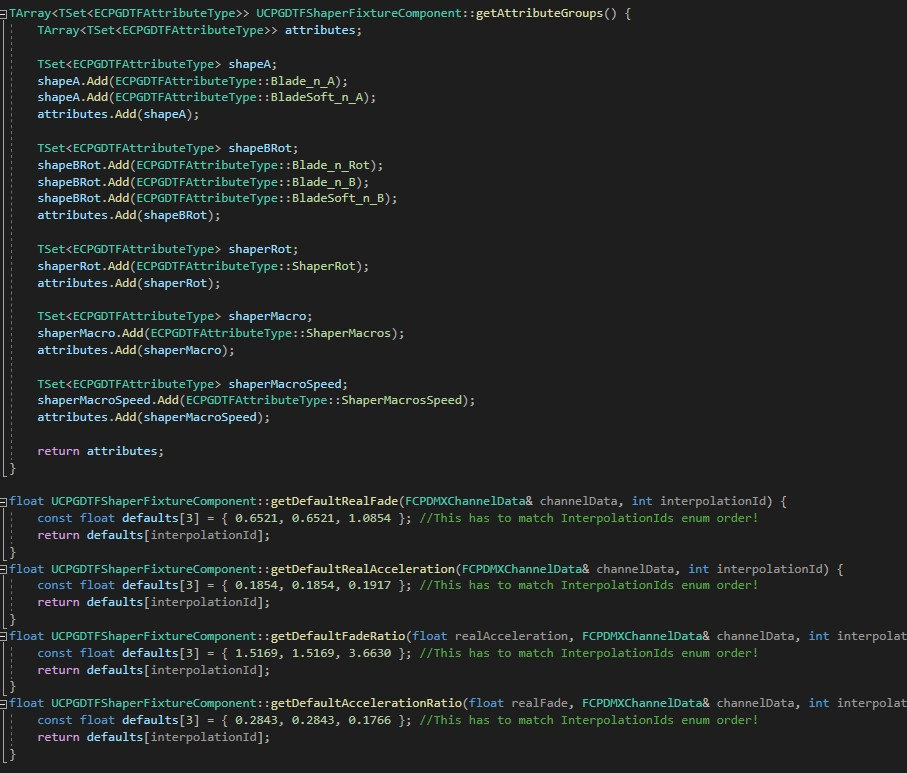
\includegraphics[width=1\linewidth]{img/newFeatures/ShaperComponentCode1.jpg}
    \label{fig:5_ShaperComponentCode1}
\end{figure}
\begin{figure}[H]
    \centering
    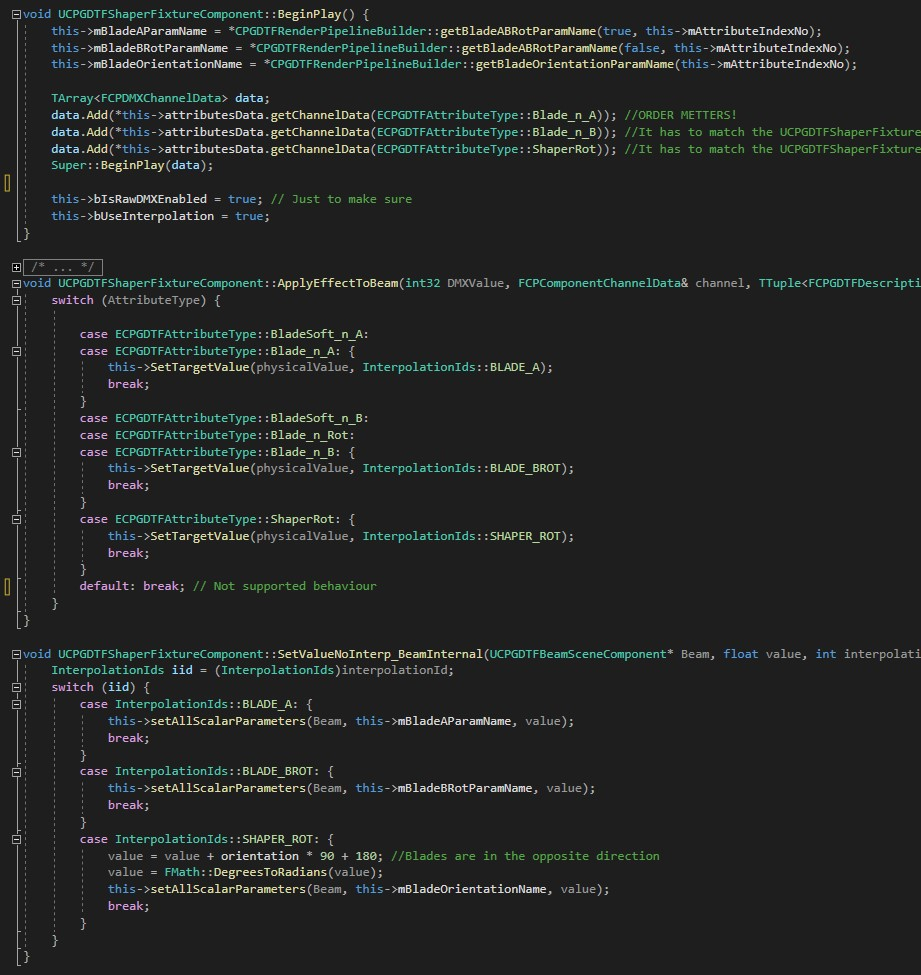
\includegraphics[width=1\linewidth]{img/newFeatures/ShaperComponentCode2.jpg}
    \label{fig:5_ShaperComponentCode2}
\end{figure}


\subsection{Iris}\label{subsec:5_Iris}
%\begin{wrapfigure}{r}{0.6\textwidth}
%    \centering
%    \captionsetup{justification=centering}
%    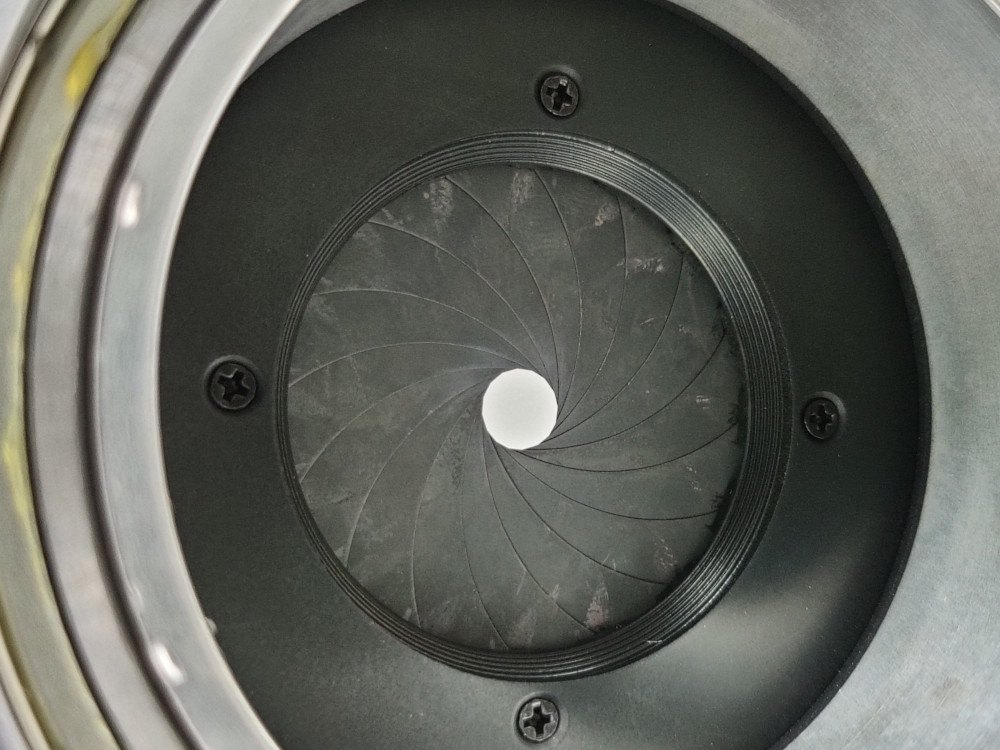
\includegraphics[scale=0.2]{img/newFeatures/Iris.jpg}
%    \caption{Modulo iris di una fixture.}
%    \label{fig:5_iris}
%\end{wrapfigure}
L'iris è una feature atta a restringere un fascio di luce. Differisce dallo zoom, poiché quest'ultimo definisce di quanto si allarga una immagine che vogliamo proiettare rispetto alla distanza, mentre l'iris definisce la dimensione in se dell'immagine. In generale, è come se fosse un sagomatore di forma circolare che entra nel fascio di luce da tutte le direzioni contemporaneamente. Così come per i sagomatori, renderizziamo questa feature attraverso formule matematiche.
\begin{figure}[H]
    \centering
    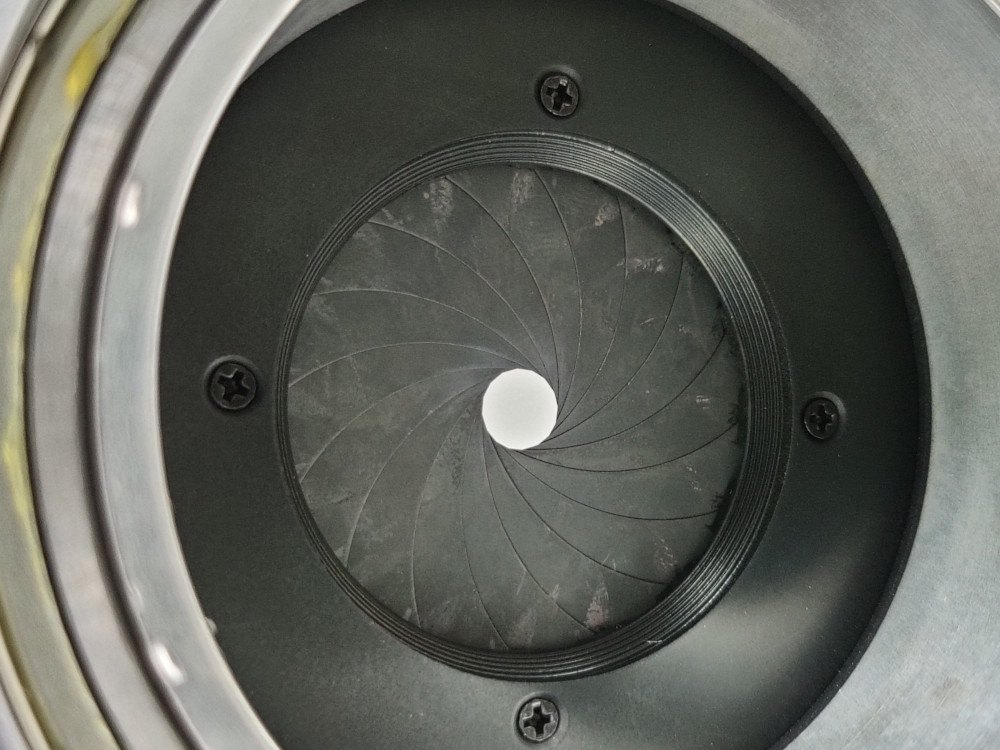
\includegraphics[width=.75\linewidth]{img/newFeatures/Iris.jpg}
    \caption{Modulo iris di una fixture.}
    \label{fig:5_iris}
\end{figure}

\subsubsection{Idea come formula matematica}\label{subsec:5_2_IrisMath}
L'idea per il rendering di questa feature è di utilizzare delle formule simili a quelle usate per il calcolo dell'area di un cerchio attraverso il metodo di Monte Carlo \cite{circleMonteCarlo}. Questo metodo consiste essenzialmente nel generare punti casuali all'interno di un quadrato le cui coordinate sono comprese tra [-1, 1], e contare quanti di questi punti cadono all'interno del cerchio e quanti all'esterno. Per sapere se un punto è collocato all'interno o all'esterno del cerchio, basta usare il teorema di Pitagora per ottenere la distanza dal centro e controllare se è più grande o piccola di 1.
\[1 > \sqrt{x^2 + y^2}\]
Per implementare l'iris, in cui abbiamo bisogno di stringere ed allargare questo cerchio, basterà controllare se la distanza è inferiore al nostro valore $i$.
\[i > \sqrt{x^2 + y^2}\]
Questa formula può essere approssimata rimuovendo interamente la radice quadrata, in modo da guadagnare un discreto incremento prestazionale. Visivamente l'iris si chiuderà in maniera esponenziale piuttosto che lineare, ma l'effetto è difficilmente notabile ad occhio nudo su un faro simulato. 
Inoltre, le coordinate UV in input sono limitate solamente al range [0, 1]. È necessario portarle nel range [-1, 1] per poter usare la formula sopra. L'equazione finale sarà quindi
\[i > (2x - 1)^2 + (2y - 1)^2\]
\newline

Per quanto riguarda il frost, si procede nella stessa maniera dei sagomatori. Si utilizza di nuovo la funzione $fade$ per ottenere l'effetto della sfocatura. La distanza ($d$) questa volta è calcolata come la differenza assoluta tra il valore dell'iris e la distanza della coordinata UV dal centro.
\[d = \abs{(2x - 1)^2 + (2y - 1)^2 - i}\]
Insorge lo stesso problema riscontrato con i sagomatori: Quando l'iris è chiuso del tutto, avere il frost attivo fa comunque apparire della sfumatura al centro del rendering. Questo problema viene risolto aggiungendo un parametro ($m$) alla $remapFrost$, che moltiplica l'intero valore della funzione:
\[remapFrost(f, m) \coloneqq m(f * 0.05 + 0.002)\]
Questo parametro per il sample dei sagomatori viene impostato ad 1, mentre per il sample dell'iris lo definiamo come uguale ad 1 se il valore dell'iris è sopra una certa soglia prefissata, altrimenti cala proporzionalmente allo stesso.
\[m = 
    \begin{dcases}
        \hfil 1 & \text{se } i \geq 0.15\\
        \frac{i}{0.15} & \text{altrimenti}
    \end{dcases}
\]

\subsubsection{Generazione codice HLSL}\label{subsec:5_2_IrisHlsl}
Le funzioni per il sample dell'iris sono state riportate in codice HLSL come segue:
\lstset{language=glsl}
\begin{lstlisting}
float sampleIris(float2 texCoor, float irisVal, float frost) {
    const float x = texCoor.x * 2 - 1, y = texCoor.y * 2 - 1;
    float dist = x * x + y * y;
    float d = abs(dist - irisVal);
    float passed = dist <= irisVal;
    const float mActivation = 0.15;
    float mEnabled = irisVal >= mActivation;
    float m = mEnabled + (1 - mEnabled) * (irisVal / mActivation);
    return fade(passed, d, frost, m);
}
\end{lstlisting}
Tale funzione è stata inserita nella struct di helper utilizzata all'interno dell'algoritmo BeamRayMarch. \newline

Nel for finale del costruttore della \lstinline{CPGDTFRenderPipelineBuilder} è stata inserita una ricerca per i componenti di tipo IrisFixtureComponent. Se vengono trovati, segnamo come vero un flag che ci dice se nella pipeline deve essere presente un iris.
\lstset{language=UEcpp}
\begin{lstlisting}
auto iris = Cast<UCPGDTFIrisFixtureComponent>(components[i]);
if (iris != nullptr) {
    hasIris = true;
    continue;
}
\end{lstlisting}

Nella generazione del codice HLSL si controlla semplicemente se tale flag è vera ed, in caso, si aggiunge il codice per il sample dell'iris, come segue:
\begin{lstlisting}
if (mIrisEnabled) {
    FString irisName = CPGDTFRenderPipelineBuilder::getInputIrisName();
    placeholderCode = placeholderCode + FString::Format(*textAdd, {
        FString::Printf(
            TEXT("sampleIris(pos.xy, %s, %s)"),
            *irisName,
            *frostVarName
        )
    });
}
\end{lstlisting}

Anche l'aggiunta alla CustomExpression del materiale Beam è molto seplice: Basta semplicemente aggiungere il parametro relativo al valore dell'iris se questo è presente.
\begin{lstlisting}
if (this->hasIris)
    addScalarInputToBeamPipeline(
        dstMaterial,
        getIrisParamName(),
        getInputIrisName(),
        meCustom, meBlocksMover
    );
\end{lstlisting}

\subsubsection{Generazione nella RenderingPipeline}\label{subsec:5_2_IrisRenderingPipeline}
Come in precedenza, la funzione $sampleIris$ è stata riportata sottoforma di MaterialFunction che prende in input il risultato del modulo precedente. Il codice che la inserisce all'interno della pipeline inizia col controllare se deve essere presente un iris.
\begin{lstlisting}
if (this->hasIris) {
    //...
}
\end{lstlisting}

Viene poi generata ed impostata la MaterialFunctionCall:
\begin{lstlisting}
MI_INIT_BLOCKS_MOVER
UMaterialExpressionMaterialFunctionCall* currentNode =
    generateMaterialExpression<UMaterialExpressionMaterialFunctionCall>(
        dstMaterial
    );
dstMaterialData->ExpressionCollection.AddExpression(currentNode);
currentNode->SetMaterialFunction(mfIris);
\end{lstlisting}
Successivamente si genera il parametro e vengono connessi gli input alla MaterialFunction.
\begin{lstlisting}
UMaterialExpressionScalarParameter* irisVal =
    addScalarParameterToMiPipeline(
        dstMaterial,
        getIrisParamName(),
        meParamsMover
    );

currentNode->FunctionInputs[1].Input.Connect(0, previousParameter);
currentNode->FunctionInputs[2].Input.Connect(0, frostParam);
currentNode->FunctionInputs[3].Input.Connect(0, irisVal);
\end{lstlisting}
Infine viene spostata la MaterialFunction ed impostata come ultimo nodo generato
\begin{lstlisting}
meModulesMover->moveMaterialExpression(currentNode);
previousParameter = currentNode;
delete meParamsMover;
\end{lstlisting}

\subsubsection{IrisFixtureComponent}\label{subsec:5_1_IrisFixtureComponent}
Il componente di gestione dell'iris, per le stesse ragioni di quello che gestisce i sagomatori, è davvero molto semplice e simile al precedente, per tanto non è necessario soffermarsi su una spiegazione generale dello stesso. L'unica cosa da tener conto è che esistono degli effetti preprogrammati all'interno delle fixture reali legati all'iris:
\begin{itemize}
    \item \textbf{Pulse}: $y = \sin^{-1}(\sin(x))$
    \item \textbf{PulseOpen}: $y = \tan^{-1}(\tan(x))$
    \item \textbf{PulseClose}: $y = -\tan^{-1}(\tan(x))$
\end{itemize}
Questi effetti sono generati e gestiti da una classe esterna (\lstinline{FPulseEffectManager}), poiché effetti simili sono di fatto disponibili anche in altre features (come ad esempio, lo shutter). I nostri compiti, da componente che si appoggia a quella classe per la generazione degli effetti pulse, sono:
\begin{itemize}
    \item \textbf{Far partire o impostare la velocità di un effetto}: questa operazione viene fatta all'interno della funzione \lstinline{ApplyEffectToBeam()} ogni qualvolta il valore dmx corrisponde ad una di queste features:
    \begin{lstlisting}
switch (AttributeType) {

    //Imposta il valore diretto dell'iris
	case ECPGDTFAttributeType::Iris:
		this->SetTargetValue(physicalValue, 0);
		break;

    //Fai partire un effetto o impostane la velocita'
    // se gia' in esecuzione
	case ECPGDTFAttributeType::IrisPulse:
	case ECPGDTFAttributeType::IrisPulseOpen:
	case ECPGDTFAttributeType::IrisPulseClose:
		if (channel.RunningEffectTypeChannel != AttributeType) 
            this->PulseManager.StartPulseEffect(
                AttributeType, 1 / physicalValue, DMXBehaviour.Key
            );
		else
            this->PulseManager.ChangePeriod(1 / physicalValue);
		break;
    default: break; // Not supported behaviour
}
\end{lstlisting}
    Dove \lstinline{StartPulseEffect()} è una funzione che si prende in input il tipo di effetto (Pulse, PulseOpen, PulseClose) selezionato
    \item \textbf{Aggiornare lo stato di un effetto}: Operazione che viene effettuata ad ogni tick dentro \lstinline{InterpolateComponent_BeamInternal}. Il nuovo stato dell'effetto viene anche usato per impostare un nuovo target dell'interpolazione.
    \begin{lstlisting}
switch (channel.RunningEffectTypeChannel) {
    case ECPGDTFAttributeType::IrisPulse:
    case ECPGDTFAttributeType::IrisPulseOpen:
    case ECPGDTFAttributeType::IrisPulseClose:
        this->SetTargetValue(
                this->PulseManager.InterpolatePulse(deltaSeconds),
            0);
        break;
    default: break;
}
\end{lstlisting}
\end{itemize}

\subsection{RenderingPipeline finale}\label{subsec:5_final}
Abbiamo mostrato nei precedenti due capitoli come l'implementazione di nuove funzionalità sia, finalmente, una operazione molto semplice e chiara, in cui definire solamente i comportamenti specifici del singolo componente.

Le seguenti immagini mostrano il risultato della generazione \say{finale} della pipeline di rendering, sia all'interno della MaterialFunction per quanto riguarda Light e Lens e sia all'interno della CustomExpression per quanto riguarda il materiale Beam.
\begin{figure}[H]
    \centering
    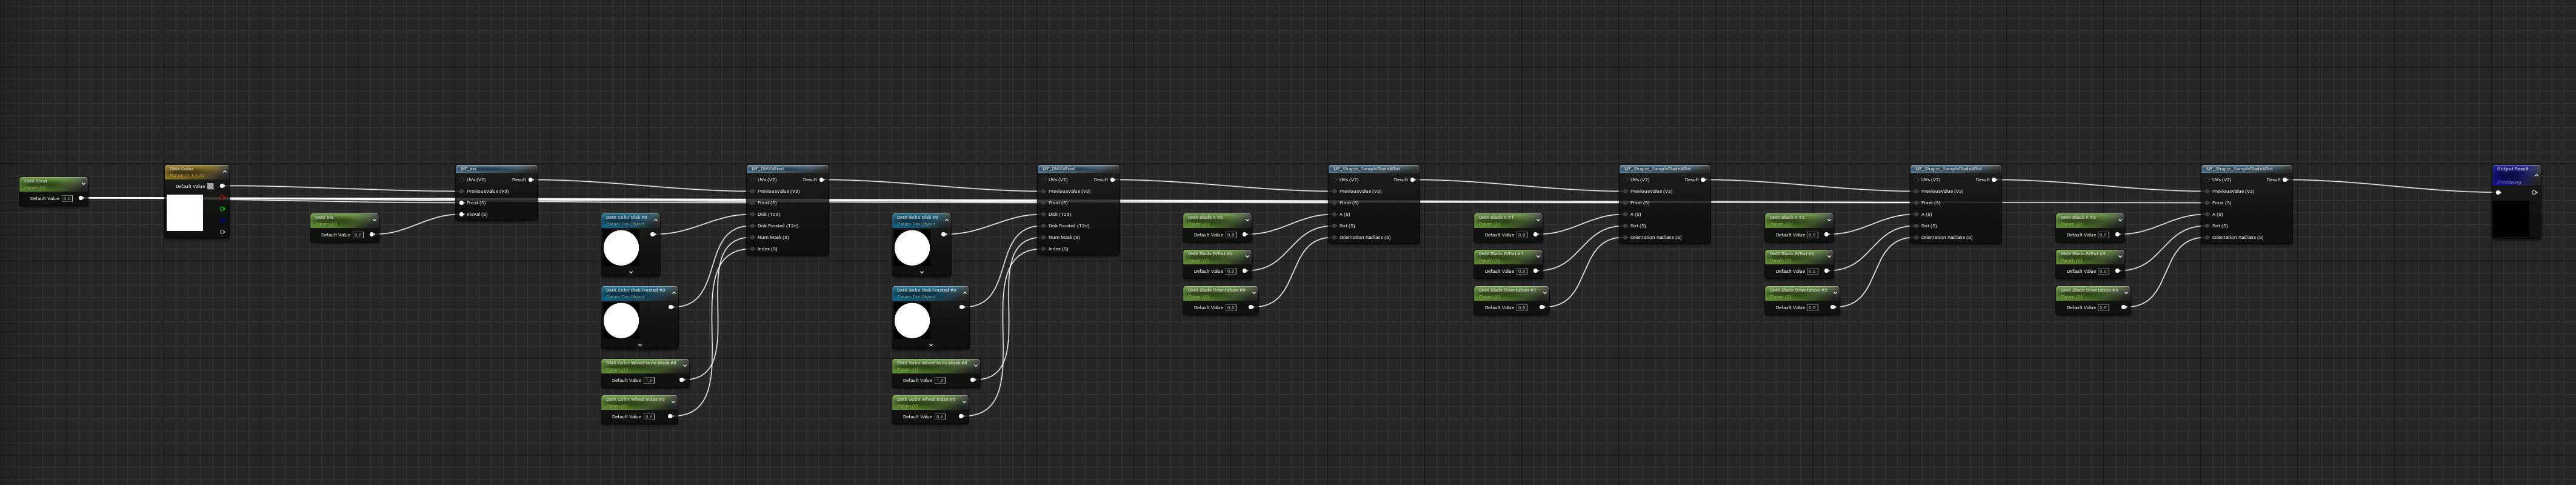
\includegraphics[width=1\linewidth]{img/newFeatures/renderPipeline.jpg}
    \caption{Rendering pipeline finale generata per i materiali Light e Lens}
    \label{fig:5_finalRenderingPipeline}
\end{figure}
\clearpage %TODO CHECK IF IT'S STILL NEEDED

Mentre il codice HLSL generato per il rendering del materiale Beam è il seguente:
\begin{lstlisting}
float3 outputSample = DMXColor; FunctionsWrapper _fncs;
outputSample = outputSample - 1 + pow(_fncs.sampleIris(
        pos.xy, irisVal, frost
), 0.66);
outputSample = outputSample - 1 + pow(_fncs.sampleWheel(
        TXTpColor__0, TXTpColor__0Sampler,
        pos.xy, NumColor__0, ColorIndex__0
), 0.66);
outputSample *= pow(_fncs.sampleWheel(
        TXTpGobo_Frosted__0, TXTpGobo_Frosted__0Sampler,
        pos.xy, NumGobo__0, GoboIndex__0
), 0.66);
outputSample = outputSample - 1 + pow(_fncs.sampleBladeARot(
        pos.xy, bladeA__0, bladeBRot__0, bladeOrientationRads__0, frost
), 0.66);
outputSample = outputSample - 1 + pow(_fncs.sampleBladeARot(
        pos.xy, bladeA__1, bladeBRot__1, bladeOrientationRads__1, frost
), 0.66);
outputSample = outputSample - 1 + pow(_fncs.sampleBladeARot(
        pos.xy, bladeA__2, bladeBRot__2, bladeOrientationRads__2, frost
), 0.66);
outputSample = outputSample - 1 + pow(_fncs.sampleBladeARot(
        pos.xy, bladeA__3, bladeBRot__3, bladeOrientationRads__3, frost
), 0.66);
\end{lstlisting}
%TODO Check if the previous code fits in just one page
\begin{figure}[H]
    \centering
    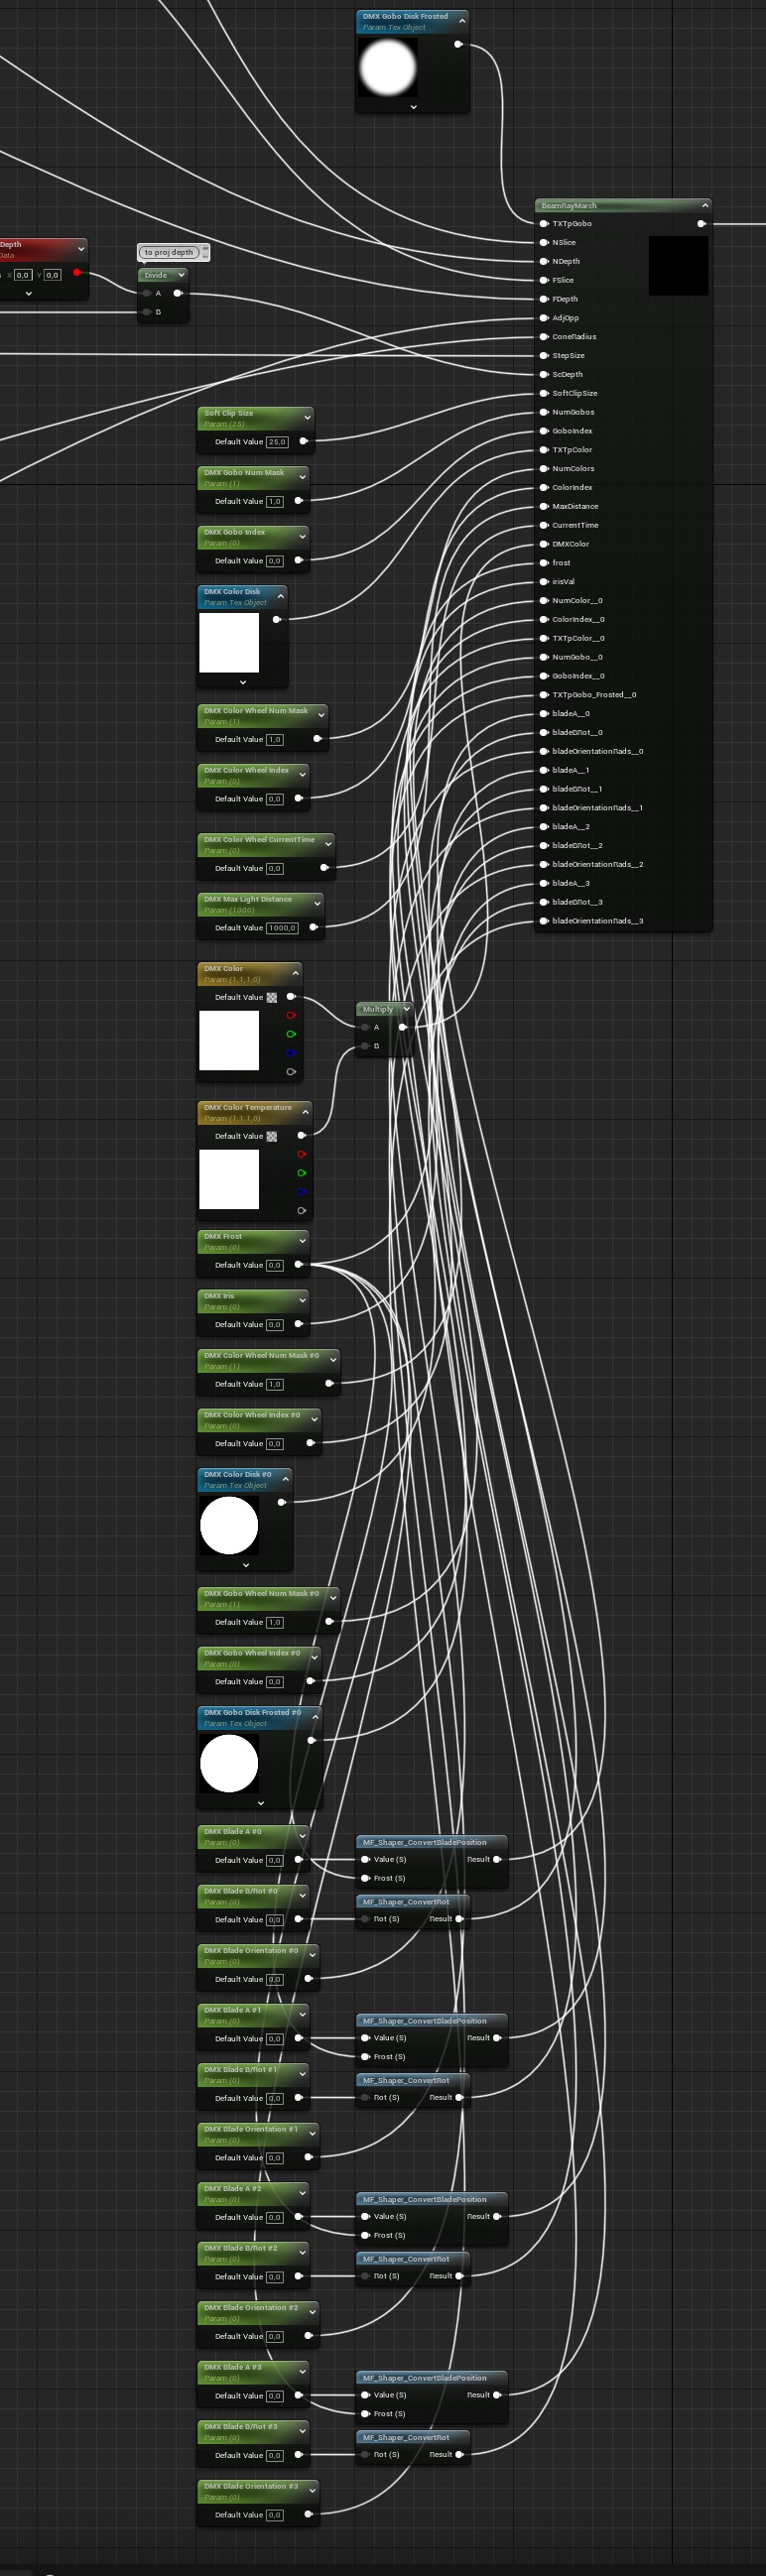
\includegraphics[width=.445\linewidth]{img/newFeatures/BeamGeneratedFull.jpg}
    \caption{Parametri per la CustomExpression per il rendering del materiale Beam}
    \label{fig:5_finalBeamCEparams}
\end{figure}

\end{document}